%%%%%%%%%%%%%%%%%%%%%%%%%%%%%%%%%%%%%%%%%%%%%%%%%%%%%%%%%%%%%%%%%
% Contents : The home chapter
% $Id : grisbi-manuel-home.tex, v 0.4 2002/10/27 Daniel Cartron
% $Id : grisbi-manuel-home.tex, v 0.5.0 2004/06/01 Loic Breilloux
% $Id : grisbi-manuel-home.tex, v 0.6.0 2011/11/17 Jean-Luc Duflot
% some of its content was in menus chapter :
% $Id: grisbi-manuel-menus.tex, v 0.5.0 2004/06/01 Loic Breilloux
% $Id : grisbi-manuel-home.tex, v 0.8.9 2012/04/27 Jean-Luc Duflot
% $Id : grisbi-manuel-home.tex, v 1.0 2014/02/12 Jean-Luc Duflot
%%%%%%%%%%%%%%%%%%%%%%%%%%%%%%%%%%%%%%%%%%%%%%%%%%%%%%%%%%%%%%%%%

\chapter{Entering Grisbi\label{entrance}}%Entrée dans Grisbi

\section{Selecting a file\label{select-file}}%Sélection d'un fichier

\vspacepdf{5mm}			% vertical space = 5 mm

When you launch the application, Grisbi displays a page allowing you to get started in different ways.%Au lancement de l'application, Grisbi affiche la page qui vous permet de démarrer de différentes manières.

\vspacepdf{5mm}			% espace : 5 mm

You can display the Grisbi window in \indexword{full screen}\index{display!full screen}\index{full screen!display} by pressing the function key \key{F11}, and go back using the same key.%Vous pouvez afficher la fenêtre de Grisbi en \indexword{plein écran}\index{affichage!plein écran}\index{plein écran!affichage} par la touche de fonction \key{F11}, et revenir en arrière par la même touche.			% "!" separates the term from the subterm of the index entry

\vspacepdf{5mm}			% espace : 5 mm

%\ifIllustration
\begin{figure}[htbp]			% h=here, t=top, b=bottom, p=page of float to force the figure here, not in a next page.
	\begin{center}					% image centrée
		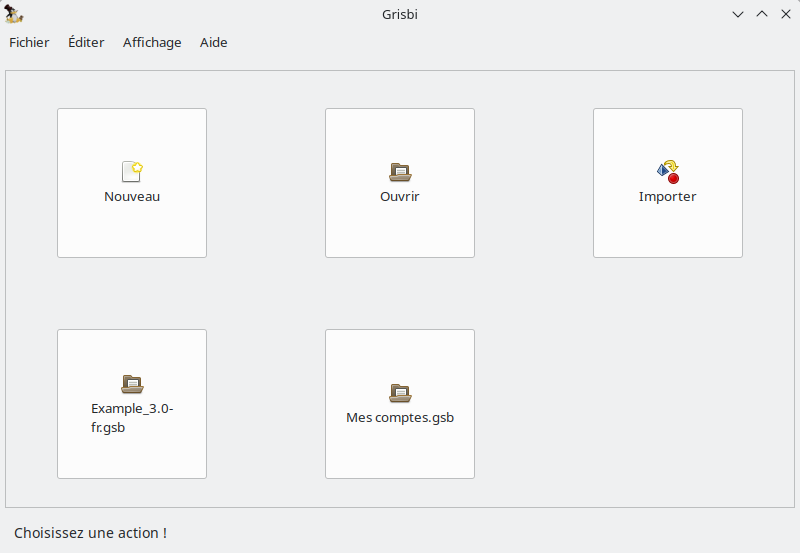
\includegraphics[width=0.95\textwidth]{image/screenshot/start_grisbi}		% width=95% as wide as the current text
	\end{center}
	\caption{Start-up window}%Fenêtre de démarrage}			% sous-titre/subtitle
	\label{start_grisbi}					% figure's ref., use for link in text with \refimage{}
\end{figure}
%\fi

\vspacepdf{3mm}			% espace : 5 mm

In addition to the menu bar, this window displays a number of panels:En plus de la barre de menu, cette fenêtre affiche plusieurs pavés:
%TODO following
\begin{itemize}
	\item le pavé Nouveau, pour lancer l'assistant \enquote{Aide à la création d'un nouveau fichier de comptes};
	\item le pavé Ouvrir, pour afficher un gestionnaire de fichier avec lequel vous pourrez chercher un fichier de comptes existant dans votre ordinateur;
	\item le pavé Importer, pour lancer l'assistant \enquote{Importation des opérations par Grisbi};
	\item un ou plusieurs autres pavés, portant le nom de fichiers de comptes que Grisbi a déjà utilisés.
\end{itemize}


\textbf{Note}: les pavés portant les noms des fichiers de comptes que Grisbi a déjà utilisés ne sont présents que si ces fichiers existent; si vous voulez les enlever de cette page d'entrée, déplacez-les dans un autre répertoire, ou supprimez-les.

\vspacepdf{5mm}			% espace : 5 mm

En bas de page, un bandeau vous appelle à choisir une action en sélectionnant l'un de ces pavés.

\vspacepdf{5mm}			% espace : 5 mm

Si vous voulez juste découvrir le logiciel Grisbi pour avoir un aperçu de son aspect et de ses possibilités, vous pouvez à la place utiliser un fichier exemple comme celui présent sur le site de \lang{Sourceforge.net}\footnote{\urlSourceForgeDocumentation{}} dans le dossier \enquote{\textsf{examples}}.		% (voir la section \vref{new-example}).

\vspacepdf{5mm}			% espace : 5 mm

\textbf{Note}: en cliquant simplement sur le fichier exemple téléchargé, Grisbi s'exécutera en affichant directement la fenêtre d'accueil\refimage{home_3.0} sans passer par la fenêtre de démarrage.



\section{Opening screen\label{home}}

\strong{Translators Note:} Until the other chapters are translated many of the cross references lead to dead-ends at the moment.


When the application starts, Grisbi displays this
%\ifIllustration
 opening screen \refimage{home-img} page.
%\else
 d'accueil.
%\fi
This opening screen can be accessed at any time by clicking on the  \menu{Accounts} tab. 

You can view the Grisbi window in \indexword{full screen mode}\index{affichage !plein écran}\index{plein écran !affichage} using the function key \key{F11}, and toggle between full screen and normal mode with the same key.

%\ifIllustration
% image centrée
\begin{figure}[htbp]
\begin{center}
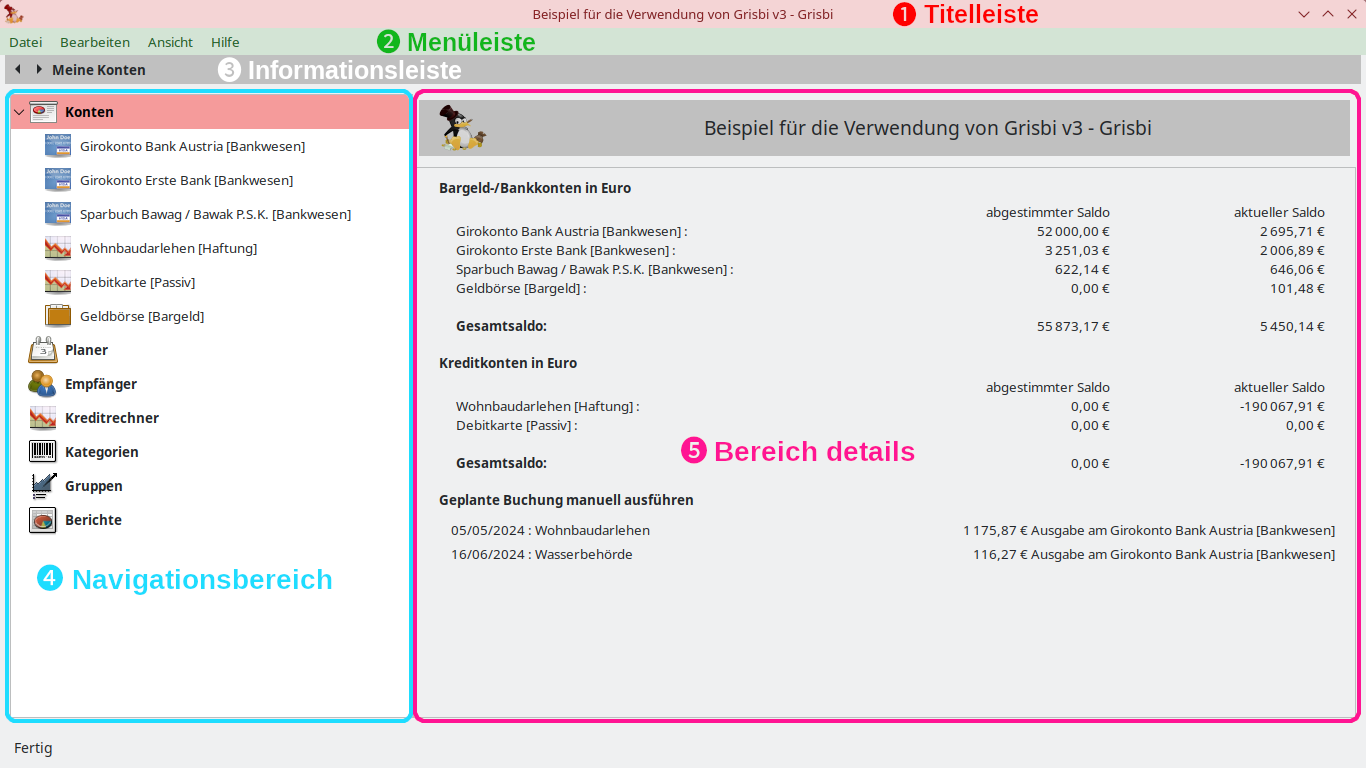
\includegraphics[scale=0.35]{image/screenshot/home_3.0.png}
\end{center}
\caption{Accounts summary page}
\label{home-img}
\end{figure}
% image centrée
%\fi

All Grisbi screens have the same general appearance. It displays a menu bar that gives access to most of Grisbi's important features, and three main areas:

\begin{itemize}
	 \item the information bar, under the menu bar;
	 \item the navigation panel;
	 \item the main screen area.
\end{itemize}

%\ifIllustration 
These three zones, specific to Grisbi, are outlined in different colors in the figure to identify them \refimage{home-img}.
%\else
%\fi

\section{Information bar\label{home-synthesis}}

The information bar displays the name of the current tab displayed, and can display, to the far right, the current balance if one of the accounts is selected for display in the main screen area.

% espace pour changement de thème
\vspacepdf{5mm}

To select one of the tabs displayed in the navigation panel click one or more times on one of the two small triangles on the top left of the panel.  The items displayed are : \menu{Accounts}, \menu{Scheduler}, \menu{Payees}, \menu{Credits simulator}, \menu{Categories}, \menu{Budgetary lines} and \menu{Reports}.  If the \menu{Accounts} and \menu{Reports} items have been expanded to display their sub categories these will also be displayed one by one.

% Pas de commande au clavier pour cette fonction
\textbf{Note} : These triangle symbols can be replaced, depending on the theme of the desktop environment or window manager you are using, by other characters such as +, -,>, <, and so on.

% espace pour changement de thème
\vspacepdf{5mm}
The content of the selection is displayed in the main screen area.

% espace pour changement de thème
\vspacepdf{5mm}
These features can be used instead of clicking directly in the navigation panel when the Information Bar window width is reduced to zero and you can not access it directly.


\section{Navigation panel\label{home-accounting}}

The navigation pane displays in bold the list of tabs:  \menu{Accounts}, \menu{Scheduler}, \menu{Payees}, \menu{Credits simulator}, \menu{Categories}, \menu{Budgetary lines} and \menu{Reports}. By clicking on the small black triangle to the left of the  \menu{Accounts} or \menu{Reports} tabs,  you can scroll or roll up the list of their sub-tabs. You can change the order of tabs and sub-tabs by clicking on one of them and dragging it up or down the list.

\textbf{Note} : These triangles can be replaced, depending on the theme of the desktop environment or window manager you are using, by other characters such as +, -,>, <, and so on.

% espace pour changement de thème
\vspacepdf{5mm}

You can select one of these tabs or sub-tabs by clicking on its name. You can also move the selection in this list of tabs and sub-tabs with the \key{Up Arrow}, \key{Down Arrow}, \key{Page Up} ou \key{Page Down} keys, or with the mouse wheel. 

% espace pour changement de thème
\vspacepdf{5mm}
The content of the selection is displayed in the main screen area.

% espace pour changement de thème
\vspacepdf{5mm}
You can reduce or enlarge the width of the navigation panel by clicking on the thin vertical bar between this panel and the main screen area, and moving it. If the width of the window has been reduced to zero, or enlarged to the maximum of the width of the Grisbi window, the thin vertical bar may be to the left or to the right of the window.  Locate this and slide it back to the desired location.

% espace pour changement de thème
\vspacepdf{5mm}

The \indexword{context menus}\index{context menus},  accessible by a right-click of the mouse, are available on the elements of this panel and offer the following functions::

\begin{itemize}
	 \item On \menu{Accounts} :
		\begin{itemize}
			 \item \menu{New account} ;
		\end{itemize}
	 \item On any account : 
		\begin{itemize}
			 \item \menu{New account},
			 \item \menu{Remove this account} ;
		\end{itemize}
	 \item On \menu{Payees} :
		\begin{itemize}
			 \item \menu{New payee},
			 \item \menu{Delete selected payee},
			 \item \menu{Edit selected payee},
			 \item \menu{Manage payees},
			 \item \menu{Remove unused payees} ;
		\end{itemize}
	 \item On \menu{Categories} : 
		\begin{itemize}
			 \item \menu{New category},
			 \item \menu{Delete selected category},
			 \item \menu{Edit selected category},
			 \item \menu{Import a file of categories (.csgb)},
			 \item \menu{Export the list of categories (.csgb)} ;
		\end{itemize}
	 \item On \menu{Budgetary lines} :
		\begin{itemize}
			 \item \menu{New budgetary line},
			 \item \menu{Delete selected budgetary line},
			 \item \menu{Edit selected budgetary line},
			 \item \menu{Import a file of budgetary lines (.isgb)},
			 \item \menu{Export the list of budgetary lines (.isgb)} ;
		\end{itemize}
	 \item On \menu{Report} : \menu{New report} ;
	 \item On any report : 
		\begin{itemize}
			 \item \menu{New report},
			 \item \menu{Remove this report}.
		\end{itemize}
\end{itemize}

%\ifIllustration
%\else
% saut de page pour titre solidaire
%\newpage
%\fi


\section{Details window\label{home-details}}

The main screen area displays all the details on the tabs or sub-tab selected by the Information Bar or Navigation Panel. This is the main work area of Grisbi.
You can reduce or enlarge its width by clicking on the thin vertical bar between this window and the navigation panel, and dragging it. If the width of the this panel has been reduced to zero or enlarged to the maximum of the width of the Grisbi window, the thin vertical bar may be to the left or to the right of the window.  Locate this and slide it back to the desired location.
 
\subsection{The summary screen\label{home-details-homepage}}

To return to the opening screen which provides an overview of the entire accounts file, select the Accounts tab; the main screen area then displays, from top to bottom:

\strong{Translators Note:} This section needs revision as the user interface is slightly different from this translation of the original French.

\begin{itemize}
	 \item in a box on a gray background, the \menu{Grisbi} icon on the left and on the right the \indexword{title}\index{title display !titre}\index{home page !page d'accueil} of the accounts file you currently have loaded, in the form   \enquote{assigned name - Grisbi} ; ??you can define this name in one of three ways the \menu{Edit preferences} menu (see the paragraph \vref{setup-display-addresses-titles}, \menu{Titles})?? ; this can be useful if you manage multiple accounting entities:

		\begin{itemize}
			 \item The \menu{Accounting Entity} : This is the name you use to identify the type of account e.g.  \enquote{My Accounts} or  \enquote{Business}, which you entered when the account file was created; you can edit it here in the   \menu{Account Name field} ; this can be useful if you manage multiple  \indexword{accounting entities}\index{entité comptable}, 
			 \item The \menu{Account holder} :the name of the owner (or  account manager) of the last account accessed; if the holder is not defined in the account properties, Grisbi displays the name of this account,
			 \item le \menu{Accounts file name} :  This is the name of the file in the current directory, in the form  \file{name\_of\_\_your\_file.gsb}, and this is the default choice;
		\end{itemize}
		
	 \item for each currency separately, for all accounts and \indexword{groups of accounts}\index{groupe de comptes},  under the label \menu{Reconciled balance} and \menu{Current balance} :
		\begin{itemize}
			 \item the balance of the bank and cash accounts, the partial balance of the groups of accounts and their Global balance,
% saut de ligne pour indentation correcte de la note dans la liste

			 \textbf{Note} : you can adjust the display order of the partial balances of the account groups (see the section \vref{setup-general-home-partBalance}, \menu{Partial balances of the list of accounts}).			 
			 \item the balance of the liability accounts and their final balance,
			 \item the balance of the asset accounts and their final balance;
		\end{itemize}
	\item the \indexword{alerts from automatically scheduled entries}\index{alerte !opération planifiée} with their date, wording and amount, according to the choices made in the \menu{Edit - Preferences menu} (see th section \vref{setup-general-planned}, \menu{Timeline}) ;
	\item the list of accounts whose balance has fallen below the  \menu{minimum authorized balance} ;
	\item the list of accounts whose balance has fallen below the  \menu{required Minimum Balance}.
\end{itemize}

% espace avant Attention ou Note  : 5 mm
\vspacepdf{5mm}


\textbf{Note} : For definitions of \menu{Minimum Allowable Balance} and \menu{Desired  minimum balance}, see the \vref{accounts-properties}, \menu{Account Properties} section.

% espace pour changement de thème
\vspacepdf{5mm}

The account labels are displayed in black{\couleur} ; as the mouse cursor moves over the line of one of these, its colour changes to gray {\couleur}.
A balance greater than the  \menu{desired Minimum Balance}  is displayed in dark green {\couleur} ; as the cursor moves over the line, its colour changes to light green {\couleur}.

A balance less than the \menu{Minimum Balance Required} and greater than the \menu{Minimum Balance authorized} is displayed in orange{\couleur} ; as the pointer passes on its line, this color changes to light orange{\couleur}.
A balance less than the  \menu{Minimum Authorized Balance}  is displayed in red{\couleur} ; as the pointer passes over its line, this color changes to light red{\couleur}.

When you move the mouse pointer over the line of an account, any color change indicates that if you click (right or left) with the mouse, the records contained in the highlighted account is displayed, as if the account had been selected with the information bar or navigation panel.

A partial balance can be specified for a group of accounts  If defined this is displayed in black{\couleur}.If it is negative, it may appear in dark red{\couleur}, (see  \vref{setup-general-home-partBalance}, \menu{Partial balances for a list of accounts}). A partial balance line does not change color when the mouse pointer is over it, because you can not view the individual entries for of an group of accounts.

% espace pour changement de thème
\vspacepdf{5mm}
You can configure certain aspects of the display of this home page in the \menu{Edit - Preferences - Main - Main Page} on the Menu Bar or in the \menu{Properties} tab of each account :
\begin{itemize}
	 \item \menu{\indexword{Fonts}\index{polices}, \indexword{logo}\index{logo} and \indexword{colours}\index{couleurs}} : section \vref{setup-display-logo} ;
	 \item \menu{?? Securities ??} : section \vref{setup-display-addresses-titles} ;
	 \item \menu{Calculation of balances} : paragraph \vref{setup-general-home-balance} ;
	 \item \menu{Partial balances from the list of accounts} : paragraph \vref{setup-general-home-partBalance} ;
	 \item \menu{Scheduler alerts} : section \vref{setup-general-planned} ;
	 \item Accounts below the \menu{\indexword{Minimum authorised balance}}\index{solde !minimal autorisé} : section \vref{accounts-properties} ;
	 \item Accounts below the \menu{\indexword{desired Minimum Balance}}\index{solde !minimal voulu} : section  \vref{accounts-properties}.
\end{itemize}

In particular, if you find a spelling error in this page, you can correct it: see the paragraph \vref{setup-general-home-final}, \menu{?? Pluriel de final ??} !

%\ifIllustration
% saut de page pour paragraphe solidaire
%\newpage
%\fi

\section{Menu bar\label{home-menus}}

As in many graphics applications, most of Grisbi's important features are accessible through the menus in the \indexword{Menu Bar}\index{barre de menus}. The features are detailed below.


\subsection{\menu{File} menu\label{home-menus-file}}

This menu includes the following functions :

\begin{itemize}
	\item \menu{New account file...} : creates a new account file; the current file is closed and a new empty file is created with an empty account (shortcut key \key{Ctrl}\key{N}),  see the \vref{start-newfile} section ; not to be confused with the creation of a new account;
	\item \menu{Open...} : open an accounts file  (shortcut key  \key{Ctrl}\key{O}) ;
	\item \menu{Recently opened files} : displays the list of the last n files opened with Grisbi (only if there have been several); this number is configurable in the \menu{Edit - Preferences}, see the \vref{setup-general-files-manage}, \menu{Account file management} section ;
	\item \menu{Save} : Saves the current account file  (shortcut key \key{Ctrl}\key{S}) ;
	\item \menu{Save as...} : opens a file manager to save the current accounts file with the name and location of your choice; Grisbi defaults to the current directory, the name of the current accounts file, with the \file{.gsb} extension ;
	\item \menu{Import file...} : starts the file import wizard of another software; see  \vref{move-import-importinit} ;
	\item \menu{Export accounts as QIF/CSV file...} : starts the Export Account File Wizard; see \vref{move-export} ;	
	\item \menu{Archive transactions...} : starts the archive creation wizard; see \vref{datamanagement-history-new} ;	
	\item \menu{Export an archive as GSB/QIF/CSV file...} : starts the archive export wizard; see \vref{datamanagement-history-export} ;
	\item \menu{Debug account file...} : starts the debug wizard for this file, which will help you look for inconsistencies in your account file; see  \vref{maintenance-file-debug} ;
	\item \menu{Obfuscate account file...} : starts the wizard that produces an anonymous copy of your account file; this file can be attached to a bug report; see \vref{maintenance-file-anonymous} ;	
	\item \menu{Obfuscate QIF file...} : starts the wizard that produces an anonymous copy of this file; this file can be attached to a bug report; see \vref{maintenance-QIF-anonymous} ;	
	\item \menu{Debug mode} : puts Grisbi in debug mode, which creates a log file of events; see \vref{maintenance-debug-mode} ; 	
	\item \menu{Close} : closes the current accounts file; Grisbi offers to save it if you have not already done it (shortcut key \key{Ctrl}\key{W}) ;
	\item \menu{Quit} : close Grisbi ; Grisbi prompts you to save the account file if you have made any changes (shortcut key \key{Ctrl}\key{Q}).
\end{itemize}


\subsection{\menu{Edit} menu\label{home-menus-edit}}

This menu includes the following functions :

\begin{itemize}
	\item \menu{Edit transaction} : see \vref{transactions-modify}, \menu{Modify a transaction} ;
	\item \menu{New transaction} : see \vref{transactions-new}, \menu{Entering a new transaction} ;
	\item \menu{Remove transaction} : see \vref{transactions-delete}, \menu{Deleting a transaction} ;
	\item \menu{Use selected transaction as a template} : see \vref{transactions-model}, \menu{Selecting a transaction for use as a template} ;
	\item \menu{Clone transaction} : see \vref{transactions-duplicate}, \menu{Clone a transaction} ;
	\item \menu{Convert to scheduled transaction} : see \vref{transactions-schedule}, \menu{Converting a transaction to a scheduled transaction} ;
	\item \menu{Move transaction to another account} : see \vref{transactions-move}, \menu{Moving a transaction to another account} ;
	\item \menu{New account} : see \vref{accounts-new}, \menu{Creating a new account} ;
	\item \menu{Remove current account} : see \vref{accounts-delete}, \menu{Removing the current account} ;
	\item \menu{Preferences} : allows you to configure Grisbi; see the \vref{setup}, \menu{Configuration of Grisbi} chapter.
\end{itemize}


\subsection{\menu{View} menu\label{home-menus-display}}

This menu includes the following functions : 

\begin{itemize}
	 \item \menu{Show transaction form} ; 
	 \item \menu{Show reconciles} (shortcut key \key{Alt}\key{R}) ;
	 \item \menu{Show lines archives} (shortcut key \key{Altl}\key{L}) ;
	 \item \menu{Show \indexword{closed accounts}}\index{compte !clos} ;
	 \item \menu{Show one line per transaction} ;
	 \item \menu{Show two lines per transaction} ;
	 \item \menu{Show three lines per transaction} ;
	 \item \menu{Show four lines per transaction} ;
	 \item \menu{Reset the column width} ; allows you to reset the columns of the tranaction lists to their original width.
\end{itemize}


\subsection{\menu{Help} menu\label{home-menus-help}}

Most of the choices in this menu give links to websites. In order for these links to work, you must have specified to Grisbi the navigation software (or browser) that you wish to use, in the \menu{Edit - Preferences} (see \vref{setup-general-programs}, \menu{Programmes}). The \menu{Help} menu includes the following choices\footnote{\strong{Translators Note:} A "help us with translation" menu item is mentioned in the French version of the manual but does note appear in the English version of Grisbi at release 1.0} :

\begin{itemize}
	\item \menu{Manual} : opens your browser to the  \enquote{Grisbi User Manual page} (shortcut key  \key{Ctrl}\key{H}) ;
	\item \menu{Quick start} : opens your browser to the  \enquote{Grisbi Quick Start page} ;
%	\item \menu{Traduction} : opens your browser to the \enquote{Translate Grisbi}, to help us to widen the internationalization of Grisbi ;
	\item \menu{About Grisbi...} : displays the program information box: you will find details about the version, the link to Grisbi's site, the acknowledgements page (contributors to the project) and the user license ;
	\item \menu{Grisbi website} : opens your browser to the \lang{Grisbi}\footnote{\urlGrisbi{}} web site ;
	\item \menu{Report a bug} : opens your browser to the \lang{Grisbi Bug Tracker page}\footnote{\urlBugTracker{}} to allow you to report a bug that you have discovered. You can also follow on this page the evolution of the corrections made to the reported bugs;
	\item \menu{Tip of the day} : opens a dialog box that displays a tip of use, different each time Grisbi starts; you can successively display all the tips, and choose whether or not the display of the tip of the day when starting Grisbi. To remove or reactivate the tip of the day, see \vref{setup-display-messages-trick}, \menu{Tip of the day}.
\end{itemize}


\section{Shortcut keys\label{home-shortcuts}}


Keyboard shortcuts make it easy to enter data and navigate through Grisbi's windows, avoiding the need to move and click. By using the ones corresponding to the most common manipulations for you, you improve your \indexword{ergonomics}\index{ergonomie} by limiting the important movements of your arms.
 
Grisbi has a number of keyboard shortcuts, presented here according to different themes (see also  \vref{introduction-manual-conventions}, \menu{Typographical conventions in this manual}).
.

\subsection{Application and files}

\begin{itemize}
	\item New accounts file : \key{Ctrl}\key{N}
	\item Open an account file : \key{Ctrl}\key{O}
	\item Register the account file : \key{Ctrl}\key{S}
	\item Close the account file : \key{Ctrl}\key{W}
	\item Close Grisbi : \key{Ctrl}\key{Q}
\end{itemize}


\subsection{Navigation panel}

\begin{itemize}
	\item Select a tab or account: \key{ Arrow Up}, \key{Arrow Down}, \key{Page Up} ou \key{Page Down}
\end{itemize}

\subsection{List of transactions and scheduled transactions}

\begin{itemize}
	\item Select a transaction: \key{Enter}
	\item Move selection:\key{Arrow Up} ou \key{Arrow Down}
	\item New transaction:  \key{Enter} on empty line, or \key{Ctrl}\key{T}
	\item Modify an transaction: \key{Enter}
	\item Delete an transaction: \key{Delete} ;
	\item Select a transaction for a reconciliation:\key{Ctrl}\key{P}
	\item Remove a reconciled transaction: \key{Ctrl}\key{R}
	\item Show or hide archival lines: \key{Altl}\key{L}
\end{itemize}


\subsection{Entry form}

\begin{itemize}
	\item The \key{Enter} is configurable : it can be set to either move in the input form, or to validate the entry
	\item Move to the next field : \key{Tab} (depending on your configuration choice)
	\item Cancel the current entry : \key{Esc}
	\item Accept auto-complete : \key{Tab} or \key{Enter} (depending on your configuration choice)
	\item  Euro symbol : \key{AltGr}\key{e}
\end{itemize}

\subsection{Drop down lists}

\begin{itemize}
	 \item Open a list : \key{Page Down} or \key{Down Arrow}
	 \item Move in the list : \key{Up Arrow}, \key{Down Arrow}, \key{Page Up} or \key{Page Down}
	 \item Validate a choice within a list: \key{Enter}
	 \item Currencies, ??exercises?? and methods of payment:
		\begin{itemize}
			\item open list : \key{Space} ; 
			\item move in the list: \key{Up Arrow} or \key{Down Arrow} ;
			\item validate the item in the list : \key{Space}.
		\end{itemize}
\end{itemize}


\subsection{Dates entered on the calendar}

\begin{itemize}
	\item Opens a calendar (on the date field) : \key{Ctrl}\key{Enter}
	\item Closes the calendar without changing the date : \key{Esc}
	\item Validate the selected date : \key{Enter}
	\item Next or previous day : \key{+} or \key{-}, \key{Right Arrow} or \key{Left Arrow}
	\item Previous or next week : \key{Up Arrow} or \key{Down Arrow}
	\item Previous or next month : \key{Page Up} or \key{Page Down}
	\item First day or last day of the month : \key{Start} or \key{End}
\end{itemize}


\subsection{Dates entered on keyboard }

\begin{itemize}
	\item Next or previous day : \key{+} or \key{-}
	\item Previous or next week : \key{Shift} \key{+} or \key{Majuscule} \key{-}
	\item Previous or next month : \key{Page Up} or \key{Page Down}
	\item Previous or Next Year : \key{Shift} \key{Page Up} or \key{Shift} \key{Page Down}
	\item Validate the selected date \key{Enter}
\end{itemize}


\subsection{Payees, categories, budget allocations, credit simulator, historical data and forecasts}

\begin{itemize}
	\item Move selection : \key{Up Arrow}, \key{Down Arrow}, \key{Page Up} or \key{Page Down}
%Ces raccourcis ne fonctionnent plus :
%	\item afficher les sous-catégories ou sous-imputations budgétaires (sur une catégorie ou une imputation budgétaire) : \key{Espace} ;
%	\item afficher les opérations des sous-catégories ou sous-imputations budgétaires (sur une sous-catégorie ou une sous-imputation budgétaire) : \key{Espace}.
\end{itemize}


\subsection{States and Configuration}

\begin{itemize}
	\item Select another tab : \key{Up Arrow}, \key{Down Arrow}, \key{Page Up}, \key{Page Down}
	\item Navigate between the tab panel and the different options in the settings panel : \key{Tab}, \key{Up Arrow}, \key{Down Arrow}, \key{Left Arrow} and \key{Right Arrow}
\end{itemize}

\subsection{Help}

\begin{itemize}
	\item Open your browser on the Grisbi User Manual page \key{Ctrl}\key{H}
\end{itemize}













